\section{Proyección inversa e imágenes de profundidad}

Al capturar una imagen con una cámara, se proyecta un fragmento del espacio sobre un plano. El proceso inverso, en el cual se estima la posición de un punto en el espacio a partir de su proyección en el plano, se llama proyección inversa o \textit{back-projection}. A partir de una imagen particular hay infinitos espacios tridimensionales que podrían reproducirla \cite{ImageReconstruction}. Por ejemplo, dos objetos de las mismas características pero distintos tamaños se podrían ver iguales en imágenes que estén a distinta distancia de la cámara. De este modo, estamos con un problema de inversas que no tiene solución única. 

En \cite{reconstruccion3DConUnaFoto} se aborda este problema con una arquitectura de red de árboles y un autoencoder a partir de una simple imagen RGB. Sin embargo, pese a que es en cierto grado posible agregando supuestos, es un proceso lento y costoso.

Para mejorar el rendimiento, se puede emplear el uso de sensores que producen imágenes de profundidad. Los mismos implementan métodos como \textit{Time of Flight} (ToF), que consiste en medir el tiempo que se tarda en emitir y recibir una luz para cada píxel. La imagen de salida se modela como una función $D: \Omega \subset Z^2 \to \mathbb{R}^+$ tal que para $(x,y)$, tenemos una representación de la distancia entre el centro óptico de la cámara y el punto real de la muestra en el espacio, medida a lo largo del rayo de visión. 

Para renderizarlas, es decir mostrarlas en la pantalla, el resultado puede definirse en una escala. Una posibilidad es en enteros entre 0 y 255, donde 255 representa los puntos que se encuentren más cercanos en la imagen, y 0 los más lejanos. Luego, podemos usar estos valores para obtener una imagen en escala de grises donde un color más claro represente una distancia menor.

\begin{figure}[H]
    \centering
    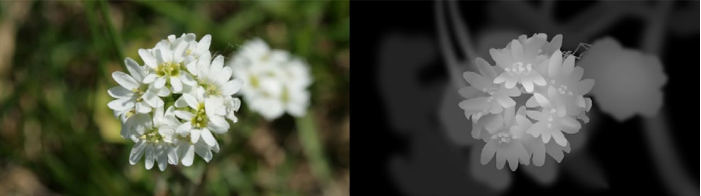
\includegraphics[width=0.8\linewidth]{../imagenes_marco_teorico/imagen_de_profundidad.png}
    \caption{A la izquierda, la imagen RGB, y a la derecha su correspondiente imagen de profundidad. Imagen extraida de \cite{imagen_de_profundidad}}
    \label{prof_imagen}
\end{figure}

En el contexto de este trabajo, se empleó una cámara RGB y una cámara de profundidad, combinación conocida como RGB-D. Debido a esto, no se profundiza en los métodos clásicos basados en la geometría epipolar, que utilizan las imágenes para obtener condiciones sobre los puntos del espacio y así definir mejor el problema. El uso de imágenes de profundidad permite basarse directamente en los datos del sensor para la estimación, a cambio de aceptar cierta cantidad de ruido y error.

Al poseer información de la profundidad, podemos invertir la relación proyectiva para obtener las coordenadas del punto en el sistema de referencia de la cámara:

\begin{equation}
\begin{pmatrix}
x \\
y \\
z
\end{pmatrix}
=
z \, \mathbf{K}^{-1}
\begin{pmatrix}
u \\
v \\
1
\end{pmatrix}.
\end{equation}

De este modo, cada píxel con información de profundidad puede asociarse a un punto
tridimensional expresado en el sistema de la cámara. Es decir, queda definido el $\lambda$ que antes desconocíamos, y el problema de inversas queda resuelto. Sin embargo, la reconstrucción sigue afectada por otros factores como el ruido, las oclusiones, y la observación incompleta del entorno. Además, desconociendo la pose de la cámara no es posible llevar la reconstrucción a coordenadas globales.